\documentclass[border=6pt]{standalone}
\usepackage{tikz}
\usetikzlibrary{arrows.meta,positioning}
\begin{document}
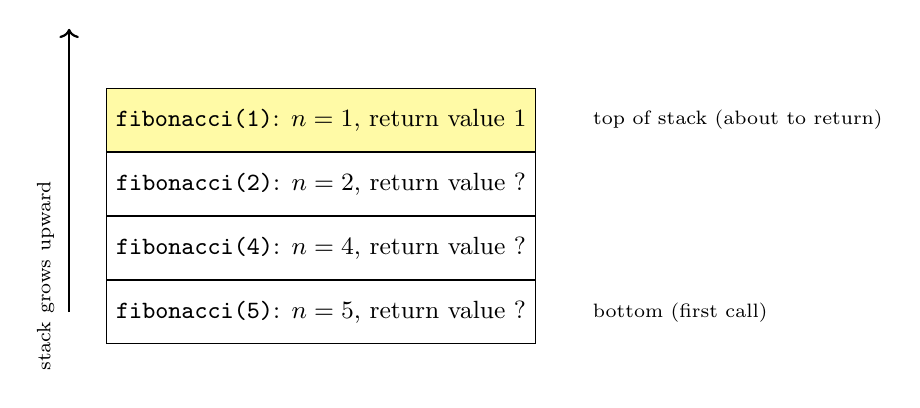
\begin{tikzpicture}[font=\small,
 rec/.style={draw,minimum width=3.6cm,minimum height=0.8cm,align=center}]
\node[rec] (r5) at (0,0) {\texttt{fibonacci(5)}: $n = 5$, return value ?};
\node[rec,above=0cm of r5] (r4) {\texttt{fibonacci(4)}: $n = 4$, return value ?};
\node[rec,above=0cm of r4] (r2) {\texttt{fibonacci(2)}: $n = 2$, return value ?};
\node[rec,above=0cm of r2,fill=yellow!35] (r1) {\texttt{fibonacci(1)}: $n = 1$, return value 1};
\node[right=0.6cm of r1,font=\scriptsize] {top of stack (about to return)};
\node[right=0.6cm of r5,font=\scriptsize] {bottom (first call)};
\draw[->,thick] (-3.2,0) -- (-3.2,3.6) node[midway,left,rotate=90,font=\scriptsize,yshift=0.3cm] {stack grows upward};
\end{tikzpicture}
\end{document}
